%%%%%%%%%%%%%%%%%%%%%%%%%%%%%%%%%%%%%%%%%%%%%%%%%%%%%%%%
\fondo{celeste}
\section{Redes convolucionales}
\fondo{blanco}
%%%%%%%%%%%%%%%%%%%%%%%%%%%%%%%%%%%%%%%%%%%%%%%%%%%%%%%%


%%%%%%%%%%%%%%%%%%%%%%%%%%%%%%%%%%%%%%%%%%%%%%%%%%%%%%%%
\begin{frame}
    \frametitle{Redes convolucionales}

    \begin{itemize}
        \item Se inspiran en la corteza visual de los animales.
        \item Desarrollo desde Neocognitron (Fukushima, 1982) a LeNet-5 (LeCun, 1989).
        \item Avance impulsado por hardware mejorado y algoritmos optimizados a partir de 2012.
        \item CNNs aplican filtros convolucionales para extraer patrones como bordes, texturas, y formas a diferentes niveles de abstracción.
    \end{itemize}

    
\end{frame}
%%%%%%%%%%%%%%%%%%%%%%%%%%%%%%%%%%%%%%%%%%%%%%%%%%%%%%%%

%%%%%%%%%%%%%%%%%%%%%%%%%%%%%%%%%%%%%%%%%%%%%%%%%%%%%%%%
\begin{frame}
\centering
    \postitimg[12cm]{Figuras/FigDL.png}
\end{frame}
%%%%%%%%%%%%%%%%%%%%%%%%%%%%%%%%%%%%%%%%%%%%%%%%%%%%%%%%


%%%%%%%%%%%%%%%%%%%%%%%%%%%%%%%%%%%%%%%%%%%%%%%%%%%%%%%%
\begin{frame}
    \frametitle{Estructura de una Red Neuronal Convolucional (CNN)}

    \begin{itemize}[leftmargin=*]
        \item \textbf{Bloque convolucional:}
        \begin{itemize}[leftmargin=*]
            \item Incluye capas de convolución, agrupamiento (pooling) y activación.
            \item Detecta patrones y características en los datos de entrada.
        \end{itemize}

        \item \textbf{Bloque totalmente conectado:}
        \begin{itemize}[leftmargin=*]
            \item Cada neurona se conecta con todas las neuronas de la capa anterior y siguiente.
            \item Correlacionan las características detectadas por las capas convolucionales.
        \end{itemize}

        \item \textbf{Bloque de decisión:}
        \begin{itemize}[leftmargin=*]
            \item Genera un vector de probabilidades para cada clase.
            \item Usa funciones como softmax.
        \end{itemize}
    \end{itemize}

\end{frame}
%%%%%%%%%%%%%%%%%%%%%%%%%%%%%%%%%%%%%%%%%%%%%%%%%%%%%%%%


%%%%%%%%%%%%%%%%%%%%%%%%%%%%%%%%%%%%%%%%%%%%%%%%%%%%%%%%
\begin{frame}[fragile]
    \frametitle{Estructura de una Red Neuronal Convolucional (CNN)}

    \begin{center}
\tikzstyle{block} = [rectangle, draw, rounded corners, minimum width=1cm, minimum height=3cm, node distance=2cm]
\begin{tikzpicture}
    % Blocks
    \node (data) {Datos};
    \node (conv) [block, right of=data, fill=green!20] {\rotatebox{90}{Bloque Convolucional}};
    \node (fc) [block, right of=conv, fill=gray!20] {\rotatebox{90}{Bloque totalmente conectado}};
    \node (softmax) [block, right of=fc, fill=red!20] {\rotatebox{90}{Bloque de decisión}};
    \node[right=of softmax] (results) {Resultados};

    % Arrows
    \draw[->] (data) -- (conv);
    \draw[->] (conv) -- (fc);
    \draw[->] (fc) -- (softmax);
    \draw[->] (softmax) -- (results);

\end{tikzpicture}
    \end{center}
\end{frame}
%%%%%%%%%%%%%%%%%%%%%%%%%%%%%%%%%%%%%%%%%%%%%%%%%%%%%%%%


%%%%%%%%%%%%%%%%%%%%%%%%%%%%%%%%%%%%%%%%%%%%%%%%%%%%%%%%
\begin{frame}[fragile]
    \frametitle{Estructura de una Red Neuronal Convolucional (CNN)}

    \begin{center}\small
\begin{tikzpicture}
    % Data block (Input)
    \node[minimum height=2.9cm, label=above:Input, minimum width=1.4cm] (data) {\rotatebox{90}{\textbf{Datos}}};
    
    % Convolutional block
    \node[draw=teal, fill=teal!10, right=0.5cm of data, minimum width=6cm, minimum height=3cm, label={[text=teal]above:Convolucional}] (convblock) {};
    
    % FC block
    \node[draw=gray, fill=gray!10, right=1cm of convblock, minimum width=1.5cm, minimum height=3cm, label={[text=gray]above:T. Conectada}] (fc) {};
    
    % Softmax block
    \node[draw=purple, fill=purple!10, right=1cm of fc, minimum width=1cm, minimum height=3cm, label={[text=purple]above:Decisión}] (softmax) {};
    
    % Convolutional layers inside convolutional block
    \node[draw=teal, minimum width=0.7cm, minimum height=2cm] (conv) at ($(convblock.west)+(0.8,0)$) {\rotatebox{90}{\color{teal}Convolución}};
    \node[draw=teal, minimum width=0.7cm, minimum height=2cm, right=0.3cm of conv] (pool) {\rotatebox{90}{\color{teal}Relleno}};
    \node[draw=teal, minimum width=0.7cm, minimum height=2cm, right=0.3cm of pool] (act) {\rotatebox{90}{\color{teal}Activación}};

    % Capa 1
    \draw[dashed, color=teal] ($(conv.west)+(-0.2,-1.3)$) rectangle ($(act.east)+(0.2,1.3)$);
    \node[below=0.5cm of pool] {\color{teal}Capa 1};
    
    % Puntos
    \node[right=0.5cm of act] (dots) {$\cdots$};

    % Capa n
    \draw[dashed, color=teal] ($(act.east)+(1.5,-1.3)$) rectangle ($(act.east)+(2.5,1.3)$);
    \node at ($(act.east)+(2,-1.8)$) {\color{teal}Capa $n$};

    % Arrow connections Convolucional
    \draw[->, thick] (data.east) -- (convblock.west);
    \draw[->, thick, teal] ($(act.east)+(0.2,0)$) -- (dots.west);
    \draw[<-, thick, teal] ($(act.east)+(1.5,0)$) -- (dots.east);

    
    % FC connections
    \node (a1) at ($(convblock.east)+(0,1)$) [inner sep=0pt]{};
    \node (a2) at ($(convblock.east)$) [inner sep=0pt]{};
    \node (a3) at ($(convblock.east)+(0,-1)$) [inner sep=0pt]{};

    \foreach \i in {-1.25,-1,...,1.25} {
        \foreach \a in {a1, a2, a3} {
            \draw[line width=0.2pt, color=gray] (\a) -- ($(fc.west)+(0.4,+\i)$);
        }
        \foreach \j in {-0.75,-0.25,...,0.75} {
            \draw[line width=0.2pt, color=gray] ($(fc.west)+(0.4,+\i)$) -- ($(fc.west)+(1.1,+\j)$);
        }
        \node at ($(fc.west)+(0.4,+\i)$) [circle, fill=gray, inner sep=1.2pt]{};
    }
    
    \foreach \j in {1,0,-1} {
        \node at ($(softmax.west)+(0.5,+\j)$) [circle, fill=purple, inner sep=1.2pt]{};
        \foreach \i in {-0.75,-0.25,...,0.75} {
            \draw[line width=0.2pt, color=purple] ($(fc.west)+(1.1,+\i)$) -- ($(softmax.west)+(0.5,+\j)$);
            \node at ($(fc.west)+(1.1,+\i)$) [circle, fill=gray, inner sep=1.2pt]{};
        }
        \draw[->, thick] ($(softmax.east)+(0,\j)$) -- ++(0.5,0);
    
    }

    % Data block (Input)
    \node[minimum height=2.9cm, minimum width=1.4cm, label=above:Output, right=0.5cm of softmax] {\rotatebox{90}{\textbf{Resultado}}};
\end{tikzpicture}
    \end{center}
\end{frame}
%%%%%%%%%%%%%%%%%%%%%%%%%%%%%%%%%%%%%%%%%%%%%%%%%%%%%%%%


%%%%%%%%%%%%%%%%%%%%%%%%%%%%%%%%%%%%%%%%%%%%%%%%%%%%%%%%
\begin{frame}
    \frametitle{Ejemplo de una CNN: LeNet-5}
    
    \centering
    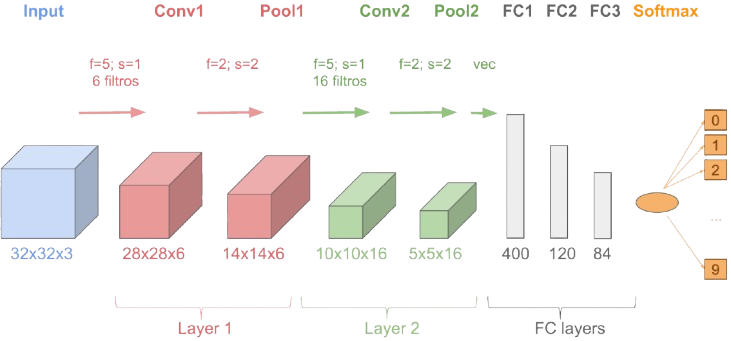
\includegraphics[width=0.9\linewidth]{Figuras/Img11.png}

\end{frame}
%%%%%%%%%%%%%%%%%%%%%%%%%%%%%%%%%%%%%%%%%%%%%%%%%%%%%%%%

%%%%%%%%%%%%%%%%%%%%%%%%%%%%%%%%%%%%%%%%%%%%%%%%%%%%%%%%
\begin{frame}
    \frametitle{Parámetros de LeNet-5}
    \centering
    \begin{tabular}{ccrr}
    \toprule
    \textbf{Capa}  & \textbf{Dimensión} & \textbf{Tamaño} & \textbf{Parámetros} \\
    \midrule
    Input   & $(32 \times 32 \times 3)$   & 3072   & 0        \\
    Conv1   & $(28 \times 28 \times 6)$   & 4704   & 456      \\
    Pool1   & $(14 \times 14 \times 6)$   & 1176   & 0        \\
    Conv2   & $(10 \times 10 \times 16)$  & 1600   & 2416    \\
    Pool2   & $(5 \times 5 \times 16)$    & 400     & 0        \\
    FC2     & $(120 \times 1)$       & 120     & 48120   \\
    FC3     & $(84 \times 1)$        & 84      & 10164   \\
    Softmax & $(10 \times 1)$        & 10      & 850      \\
    \midrule
    Total &&&62006\\
    \bottomrule
    \end{tabular}

\end{frame}
%%%%%%%%%%%%%%%%%%%%%%%%%%%%%%%%%%%%%%%%%%%%%%%%%%%%%%%%

%%%%%%%%%%%%%%%%%%%%%%%%%%%%%%%%%%%%%%%%%%%%%%%%%%%%%%%%
\begin{frame}
    \frametitle{Transferencia del Aprendizaje}

    \begin{itemize}[leftmargin=*]
        \item Permite reutilizar un modelo entrenado en una tarea para aplicarlo en otra tarea similar.
        \item Mejora el rendimiento del modelo y acelera el progreso.
        \item Es popular en \textbf{Deep Learning} debido a los altos costos computacionales y de datos necesarios para entrenar modelos desde cero.
        \item La técnica más común es usar un \textbf{modelo pre-entrenado} y adaptarlo:
        \begin{itemize}
            \item Seleccionar el modelo fuente.
            \item Reutilizar todo o parte del modelo.
            \item Ajustar el modelo a la nueva tarea (fine-tuning).
        \end{itemize}
    \end{itemize}

\end{frame}
%%%%%%%%%%%%%%%%%%%%%%%%%%%%%%%%%%%%%%%%%%%%%%%%%%%%%%%%

%%%%%%%%%%%%%%%%%%%%%%%%%%%%%%%%%%%%%%%%%%%%%%%%%%%%%%%%
\begin{frame}
    \frametitle{¿Y en la práctica?}

    \begin{block}{}
        \centering
        Con redes convolucionales y transferencia del aprendizaje disponemos
        de herramientas muy poderosas para analizar imágenes.
    \end{block}

    \pause
    \vspace{0.4cm}
    \begin{alertblock}{}
        \centering
        Con esta ideas, podemos \textbf{detectar polinizadores en imágenes de flores}.
    \end{alertblock}

\end{frame}
%%%%%%%%%%%%%%%%%%%%%%%%%%%%%%%%%%%%%%%%%%%%%%%%%%%%%%%%
